% begin module polynomials
\begin{frame}
\frametitle{Polynomials}
\begin{definition}[Polynomial Function]
A polynomial function is a function $f$ of the form
\[
f(x) = a_0 + a_1x + a_2x^2 + \cdots + a_{n - 1}x^{n-1} + a_nx^n ,
\]
where $n$ is a non-negative integer and $a_0, \ldots , a_n$ are real numbers, called the coefficients. If $a_n\neq 0$ the integer $n$ is called the degree of $f$.

\only<1>{~\\~\\If we interpret $x$ as an indeterminate formal expression, rather than a number, we say that $f(x)$ is a polynomial (rather than a polynomial function).}

\end{definition}
\uncover<2->{
\[
\begin{array}{|c|c|c|c|c|c|}
\hline
f(x) &%
\alert<handout:0| 3-4,13-14,23-26,35-36>{\text{Polynomial?}} &%
\alert<handout:0| 5-6,15-16,27-28>{\text{Degree}} &%
\alert<handout:0| 7-8,17-18,29-30>{a_0} &%
\alert<handout:0| 9-10,19-20,31,32>{a_1} &%
\alert<handout:0| 11-12,21-22,33-34>{a_2} \\
\hline
\alert<handout:0| 3-12>{x^4-x+1} &%
\uncover<4->{\alert<handout:0| 4>{\text{Yes}}}&%
\uncover<6->{\alert<handout:0| 6>{4}}&%
\uncover<8->{\alert<handout:0| 8>{1}}&%
\uncover<10->{\alert<handout:0| 10>{-1}}&%
\uncover<12->{\alert<handout:0| 12>{0}}\\%
\alert<handout:0| 13-22>{6} &%
\uncover<14->{\alert<handout:0| 14>{\text{Yes}}}&%
\uncover<16->{\alert<handout:0| 16>{0}}&%
\uncover<18->{\alert<handout:0| 18>{6}}&%
\uncover<20->{\alert<handout:0| 20>{0}}&%
\uncover<22->{\alert<handout:0| 22>{0}}\\%
\alert<handout:0| 23>{3x^2 - \frac{1}{2}x + \alert<handout:0| 24>{\sqrt{x}}} &%
\uncover<24->{\alert<handout:0| 24>{\text{No}}}&%
&%
&%
&\\
\alert<handout:0| 25-34>{3x^2 - \frac{1}{2}x + \sqrt{2}} &%
\uncover<26->{\alert<handout:0| 26>{\text{Yes}}}&%
\uncover<28->{\alert<handout:0| 28>{2}}&%
\uncover<30->{\alert<handout:0| 30>{\sqrt{2}}}&%
\uncover<32->{\alert<handout:0| 32>{-\frac{1}{2}}}&%
\uncover<34->{\alert<handout:0| 34>{3}}\\%
\alert<handout:0| 35>{3x^2 - \frac{1}{2\alert<handout:0| 36>{x}} + \sqrt{2}} &%
\uncover<36->{\alert<handout:0| 36>{\text{No}}}&%
&%
&%
&\\
\hline
\end{array}
\]
}
\end{frame}


\begin{frame}
\begin{itemize}
\item<1->  Linear functions are polynomial (functions).
\item<2->  So are quadratic functions.  Their graphs are parabolas.
\item<3->  And there are many more.
\end{itemize}
\only<handout:1| 1>{%
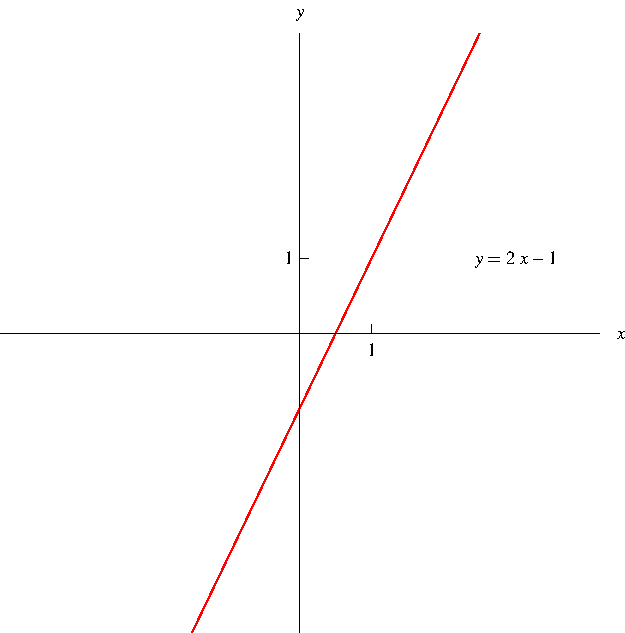
\includegraphics[height=6cm]{precalculus/pictures/01-02-line.pdf}%

Linear
}%
\only<handout:2| 2>{%
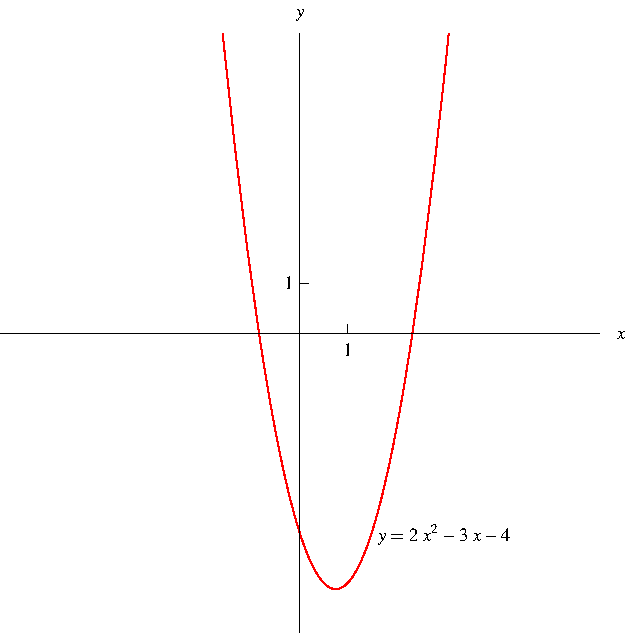
\includegraphics[height=6cm]{precalculus/pictures/01-02-parabola.pdf}%

Quadratic
}%
\only<handout:3| 3>{%
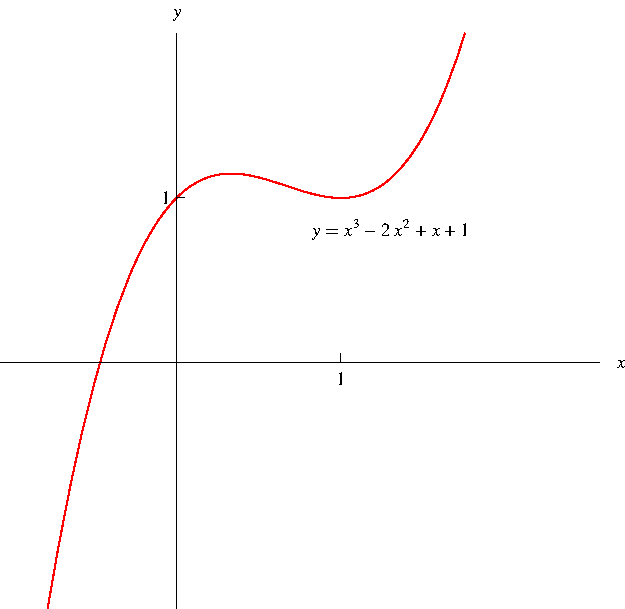
\includegraphics[height=6cm]{precalculus/pictures/01-02-polya.pdf}%

Cubic
}%
\only<handout:4| 4>{%
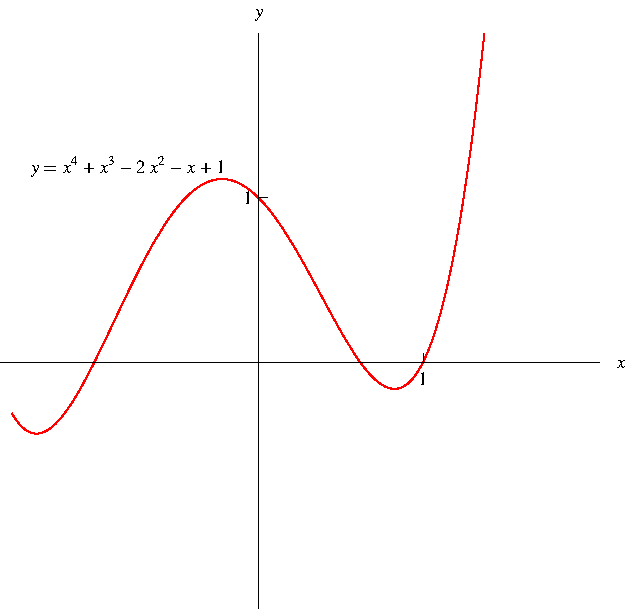
\includegraphics[height=6cm]{precalculus/pictures/01-02-polyb.pdf}%

Quartic
}%
\only<handout:5| 5>{%
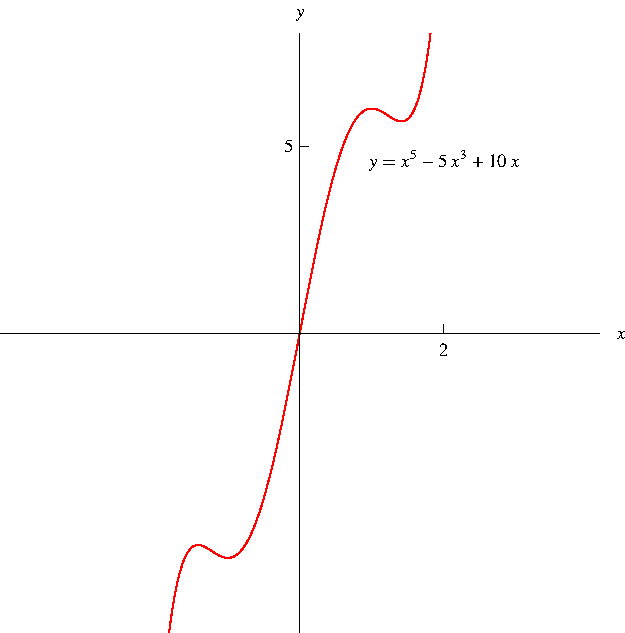
\includegraphics[height=6cm]{precalculus/pictures/01-02-polyc.pdf}%

Quintic
}
\end{frame}
% end module polynomials
